% !TEX program = lualatex
% MHM2010 Correction Workbench documentation
% Version: 0.1.0 | Author: William W. Wallace | Created/Modified: 2026-11-03
% Revision: 0.1.0 Initial operator manual, validation and equation appendix.
% Build twice: lualatex -interaction=nonstopmode -halt-on-error <this file>
\documentclass[11pt,a4paper]{article}
\usepackage[margin=19mm,headheight=16pt]{geometry}
\usepackage{fontspec}
\setmainfont{TeX Gyre Pagella}
\setsansfont{TeX Gyre Heros}
\setmonofont{Latin Modern Mono}[Scale=0.88]
\usepackage{amsmath,amssymb,booktabs,longtable,array,graphicx,xcolor}
\usepackage{enumitem,fancyhdr,listings,xurl}
\usepackage[unicode,colorlinks=true,linkcolor=teal,urlcolor=teal,
  bookmarksopen=true,bookmarksnumbered=false,pdfpagelabels=true]{hyperref}
\usepackage{bookmark}
\definecolor{navy}{HTML}{172C40}
\definecolor{teal}{HTML}{176B79}
\definecolor{light}{HTML}{EFF5F7}
\setcounter{secnumdepth}{0}
\setcounter{tocdepth}{1}
\setlength{\emergencystretch}{2em}
\setlength{\parindent}{0pt}
\setlength{\parskip}{6pt}
\setlist[itemize]{leftmargin=5mm,itemsep=3pt,topsep=3pt}
\pagestyle{fancy}
\fancyhf{}
\fancyhead[L]{\sffamily\small MHM2010 / CORRECTION WORKBENCH}
\fancyhead[R]{\sffamily\small 0.1.0}
\fancyfoot[L]{\sffamily\footnotesize Offline engineering analysis}
\fancyfoot[R]{\sffamily\footnotesize\thepage}
\renewcommand{\headrulewidth}{0.4pt}
\hypersetup{pdftitle={MHM2010 Correction Workbench: Operator and Scientific Manual},
 pdfauthor={William W. Wallace},pdfsubject={Version 0.1.0, Python 3.12, both masermon drift units}}
\lstset{basicstyle=\ttfamily\small,breaklines=true,frame=single,
 backgroundcolor=\color{light},rulecolor=\color{teal},columns=fullflexible}
\newcommand{\manual}{\href{https://www.gb.nrao.edu/~fghigo/timer/MSMmaser/Maser_UG_75666-201_Rev_J.PDF}{[1]}}
\newcommand{\nist}{\href{https://tf.nist.gov/general/pdf/2220.pdf}{[2]}}
\newcommand{\stablemanual}{\href{http://www.stable32.com/Manual154.pdf}{[3]}}
\newcommand{\siteclock}{\href{https://www.gb.nrao.edu/~fghigo/timer/time_logging.html}{[4]}}
\newcommand{\warning}[1]{\par\noindent\colorbox{light}{\parbox{\dimexpr\linewidth-2\fboxsep}{\textbf{Review boundary.} #1}}\par}
\begin{document}
\begin{titlepage}
\pdfbookmark[0]{Title}{title}
{\sffamily\color{teal}\large PRECISION TIMING / ENGINEERING SOFTWARE\par}
\vspace{18mm}
{\sffamily\color{navy}\Huge MHM2010\\Correction Workbench\par}
\vspace{5mm}
{\sffamily\Large Operator and Scientific Manual\par}
\vspace{9mm}
\rule{\linewidth}{1pt}
\vspace{5mm}
{\large FITS-first timing analysis, HMD telemetry, interactive fitting,\\
two masermon drift-unit representations, stability and native Veusz output.\par}
\vspace{12mm}
\begin{tabular}{@{}ll@{}}
Application version & 0.1.0\\
Bundled writer & \texttt{vszh5\_writer.py} 0.0.22\\
Author & William W. Wallace\\
Date & November 3, 2026\\
Runtime & Python 3.12\\
GUI & qtpy / PySide6 / pyqtgraph\\
License & GPL-3.0-or-later\\
\end{tabular}
\vfill
\warning{This application does not control a maser. Numerical candidates are
advisory and require verification of current DDS, drift state, sign convention,
reference behavior and application epoch. Historical examples are not settings
to enter today.}
\vspace{5mm}
{\small Deliverable contract: runnable source; live interval fitting; both drift
units; FITS and Franks timing inputs; HMD context; stability; Stable32; native
\texttt{.vszh5}; bookmarked PDF and editable LuaLaTeX; tested examples and a 7z package.
Physical instrument certification is outside this release.}
\end{titlepage}
\pdfbookmark[0]{Contents}{contents}
\tableofcontents
\clearpage

\section{Purpose and verified instrument relationship}
The instrument mapping follows the MHM2010 manufacturer's guide \manual;
stability definitions follow NIST SP 1065 \nist; and interchange files follow
the Stable32 manual \stablemanual. These references establish the analytical
framework, not a certification of the installed system.

The workbench estimates residual maser-to-reference fractional frequency and
frequency drift from measured timing offsets. Housekeeping telemetry identifies
instrument context and changes; it is not an independent frequency reference.
The Green Bank system logs switched one-pulse-per-second comparisons involving
Site1Hz, MicroSem and GPS channels \siteclock.

The MHM2010 manual gives the exact relationship between maser oscillation
frequency, the external synthesizer number and the standard output frequency.
An increase in the synthesizer number lowers output frequency; the nominal
calibration is \(7.04024\times10^{-17}\) per least-significant displayed digit
\manual. The application derives its local gain from the exact denominator,
rather than treating the nominal calibration as exact.

The supplied screenshot identifies the two target controls as \textbf{External
DDS Setting} and \textbf{Drift Correction}. The manufacturer's manual explicitly
offers \textbf{DDS Units/day} and \textbf{pp \(10^{18}\)/day} in the drift control
\manual. Both are computed simultaneously in this release.

\begin{longtable}{@{}p{.31\linewidth}p{.64\linewidth}@{}}
\toprule
Documented item & Treatment in this release\\
\midrule
DDS versus output direction & Increasing DDS decreases output frequency \manual.\\
DDS precision & One displayed last digit is \(10^{-7}\) in the synthesizer number \manual.\\
Drift-unit choices & Both DDS units/day and parts in \(10^{18}\)/day are available \manual.\\
External control & Front-panel synthesizer selection must permit external control \manual.\\
Drift-field sign & Not explicitly stated in inspected Rev. J; user selects and verifies it.\\
Numeric limits and cadence & Not specified in inspected Rev. J; not invented by this program.\\
Housekeeping selector codes & Retained as raw logged values; not decoded into an enable assertion.\\
\bottomrule
\end{longtable}

\warning{A phase offset cannot be removed merely by selecting a zero steady
frequency error. This software does not plan phase slews or write the
instrument. It estimates slope and curvature and leaves the constant phase
offset unchanged.}

\subsection{Release structure}
\begin{itemize}
\item \textbf{Application}: GUI entry point plus separate input, science and export modules.
\item \textbf{Batch path}: \texttt{analyze\_maser.py} accepts explicit paths and historical assumptions.
\item \textbf{Writer}: the supplied native h5py writer, with a targeted date-shape fix.
\item \textbf{Documentation}: this PDF, its LuaLaTeX source, README, changelog and validation report.
\item \textbf{Examples}: a 30-day historical result with raw pair datasets, reports and Stable32 output.
\end{itemize}
\clearpage

\section{Installation and first run}
Use Python 3.12 in an isolated environment. No fixed personal directory names
are embedded in the application. Run the following inside the extracted package:
\begin{lstlisting}
py -3.12 -m venv .venv
.\.venv\Scripts\python.exe -m pip install -r requirements.txt
.\.venv\Scripts\python.exe MHM2010_Correction_App.py
\end{lstlisting}

The supplied Windows launcher uses the adjacent environment if present,
otherwise Python's 3.12 launcher. Source files have author/revision headers,
semantic versions, Spyder cell markers and explanatory comments. In Spyder,
select the same environment; a dedicated console is preferable if a GUI loop
is already active.

The default backend is PySide6 through qtpy. The application does not import
PySide6 directly. pyqtgraph is configured to match the selected Qt backend.
PyQt6 may be selected explicitly through \texttt{QT\_API}, but that alternate
backend was not validated for this release.

\subsection{Dependencies and offline behavior}
The runtime requirements are NumPy, SciPy, pandas, Astropy, h5py, QtPy,
PySide6 and pyqtgraph. The supplied environment-version list records the
packages used for testing. Installing dependencies requires package access;
the scientific analysis itself requires no web service, API key, instrument
socket or serial connection.

Veusz is optional for viewing or rendering output, not for generating
\texttt{.vszh5}. Test dependencies include pytest and AllanTools. The included
manual was compiled with LuaLaTeX; run the command twice from the docs folder:
\begin{lstlisting}
lualatex -interaction=nonstopmode -halt-on-error MHM2010_Workbench_Manual_v0.1.0.tex
\end{lstlisting}

\subsection{Quick workflow}
\begin{enumerate}[leftmargin=6mm,itemsep=4pt]
\item Select raw OnePpsDeltas FITS/FITS.GZ files using the GUI or drag-and-drop.
\item Load HMD housekeeping separately; select the intended MicroSem/GPS pair.
\item Choose a continuous acquisition run and a clean fit interval.
\item Compare linear and quadratic behavior and inspect residuals and other references.
\item Enter the DDS and enabled drift at the intended application epoch.
\item Verify signs and operating state; inspect both drift-unit representations.
\item Compute stability with an explicit sampling tolerance and detrending choice.
\item Export to a new results folder and retain the source hashes and review record.
\end{enumerate}

\warning{This release was tested in a Linux cloud environment. Actual Windows
file dialogs, display scaling, Stable32 application import and physical
maser operation remain untested. No connected bracca device was exposed at the
last inventory check, so local staging was not performed.}
\clearpage

\section{Input data and provenance}
\subsection{Preferred input: raw OnePpsDeltas FITS}
The parser requires the \texttt{OnePpsDeltas} binary table with \texttt{DMJD},
\texttt{CHANNELA}, \texttt{CHANNELB} and \texttt{DELTAT}. It verifies UTC time
metadata and declared time/phase units. Files marked simulated are rejected.
Blank channel names, nonpositive timestamps and padding rows are rejected.
FITS \texttt{TNULL} values are honored when supplied.

Every measured channel pair stays separate. The direct
\texttt{MicroSem -> CNS\_GPS1} pair is preferred over subtracting sequential
Site1Hz observations. Reverse-direction pairs are not merged into the direct
pair: their measurements occur at different times and can include fixed
channel-path asymmetries. Valid raw zero values and \(-9999\) ns observations
are not automatically treated as missing.

Rows are sorted by timestamp. Identical duplicates are removed and counted;
different values at one identical pair timestamp cause a failure rather than
an arbitrary choice. The parser records input basenames, sizes and SHA256
hashes, without exporting personal absolute directory paths.

\subsection{Alternative input: Franks t00new}
Franks files are reduced timing data. The parser locates the named MJD header,
requires the nanosecond declaration and preserves each available timing column.
Values \(-9999\) and the historical \(-999\) sentinel are removed in this adapter
only. Raw FITS and reduced Franks files cannot be loaded as one combined batch.

Hourly median timestamps are often irregular. They can be fitted using actual
timestamps, but cannot automatically be treated as a uniform stability record.
The original reduction windows and raw samples cannot be recovered from the
reduced values.

\subsection{HMD telemetry}
HMD is parsed as a timestamped comma-delimited table. It must include MJD and
the external synthesizer column. All numeric housekeeping channels remain
available for display. Large discrete DDS changes and selector-code changes
are marked as candidate events; gradual drift ramps are not called steps.

The event detector uses a configurable function argument with a GUI default
of 50 least-significant DDS digits. This is an application heuristic, not a
manufacturer alarm threshold. Alarm/status channel voltages remain raw
values. Missing HMD coverage is reported; historical telemetry is never silently
used as the current state at an unrelated epoch.

\subsection{Timing overview and the supplied Veusz exemplar}
The overview creates UTC-hour medians for available Site1Hz comparisons,
direct MicroSem/GPS measurements and a separately labeled difference of
Site1Hz medians. All raw measured pairs remain in the export. Missing channels
such as RA or TAC are not fabricated.

Each available overview channel has MJD and proper UTC-axis export pages.
This reproduces the useful dataset families in the supplied Franks Veusz
example without copying its all-missing channels or invalid legacy dates.
UTC-hour binning is not claimed identical to the historical reduction windows.
\clearpage

\section{Interactive analysis}
\begin{center}
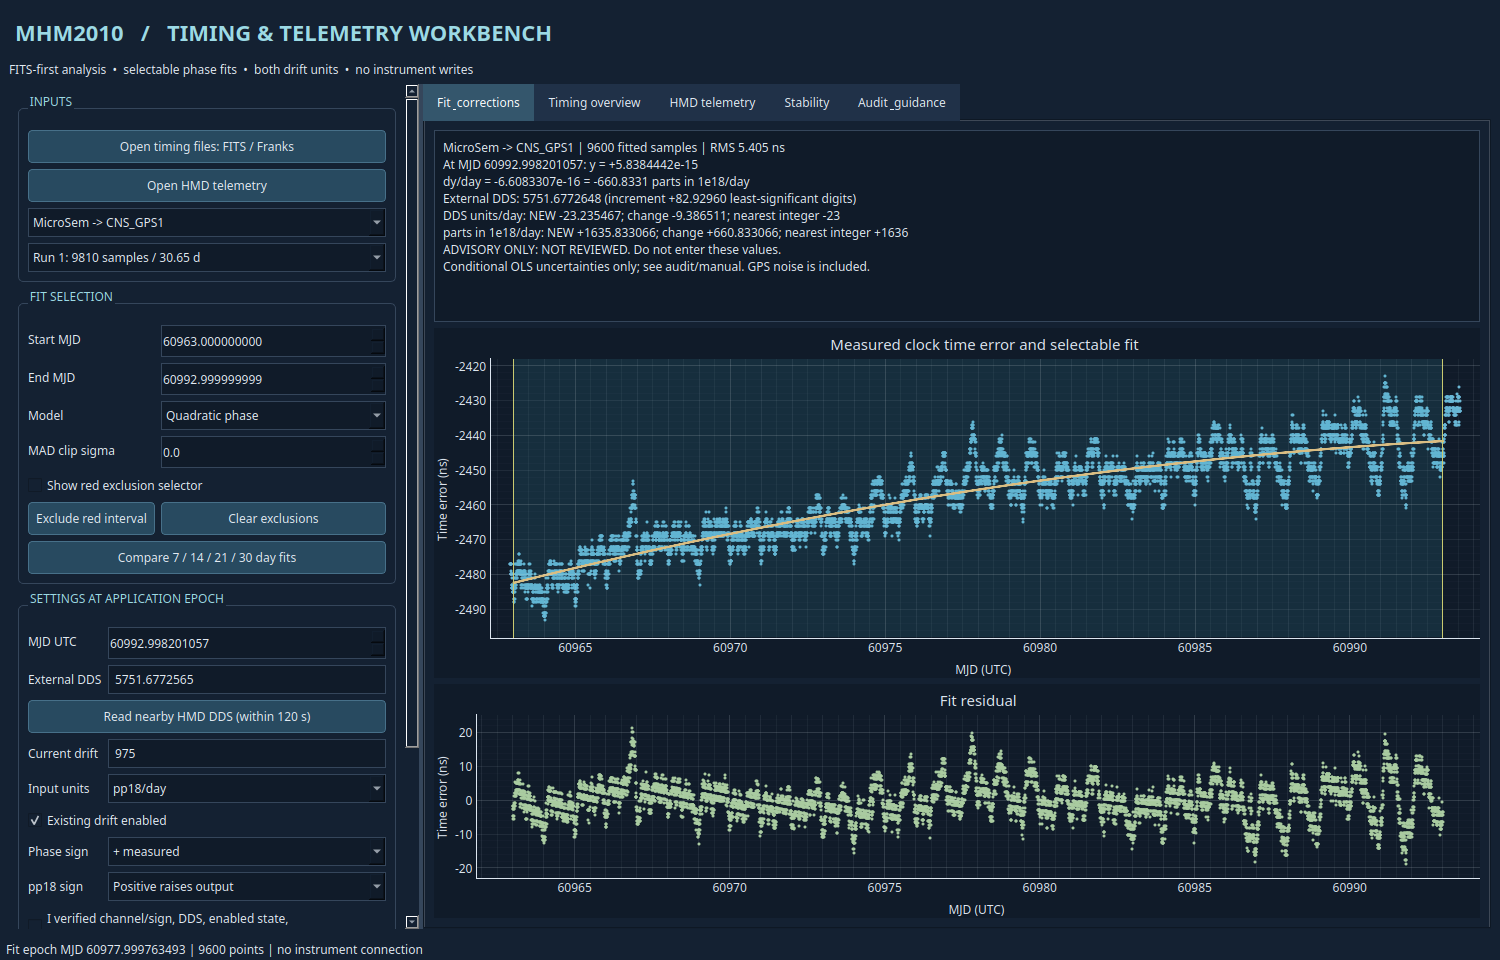
\includegraphics[width=\linewidth]{../validation/gui_fit.png}
\end{center}
\smallskip
\textbf{Fit and corrections tab.} The blue region selects the fitting interval.
The phase and residual plots share their horizontal view. Numeric MJD limits
provide precise selection without requiring a mouse.

The red region is an independent exclusion selector. Add its interval to the
exclusion list or clear the list. Excluded observations remain in the input
and export, with an explicit used-in-fit mask. Optional iterative MAD residual
clipping is disabled by default. It can reject outliers, but it changes noise
statistics and must not conceal physical events.

A linear phase model estimates frequency only; the drift field is not
estimated and should not be changed on that basis. A quadratic phase model
estimates frequency and frequency drift. Internal scaling improves numerical
conditioning without changing the physical units of the returned coefficients.

The 7/14/21/30-day comparison button reports trailing-window fits in the audit
tab. These are unclipped quadratic diagnostic fits, with actual span and
sample count shown. They are not confidence intervals.

\subsection{State and stale-result handling}
Changing the fit interval/model invalidates old stability results. Settings
can be saved without source-directory paths, then restored after selecting the
original files. Restoring settings clears operator acknowledgments. Export
creates a new folder; it never silently replaces an earlier result directory.

\warning{The plots are interactive analysis of selected files, not streaming
acquisition. Large file reads run outside the GUI thread; fitting, overview
construction and export may briefly occupy the GUI thread for very large
datasets. There is no serial or network maser interface in this release.}
\clearpage

\section{Correction interpretation and manual review}
\subsection{One epoch, two absolute settings}
The phase fit is centered on an internal reference epoch. Frequency error is
evaluated at the separate intended application epoch. The old DDS must be the
setting at that application epoch, not the setting at the start of the data
or at the centered fit epoch.

The new external DDS is an \textbf{absolute setting}, not a number to add
again. Its displayed increment is also reported in least-significant DDS
digits. The new drift is the existing enabled drift plus a residual correction,
with the sign and units handled explicitly. An existing disabled drift
contributes zero regardless of a stale numeric value in its field.

The pp18/day input field and DDS-units/day input field are alternative
representations of the same ramp. The program reports both new values and
both increments. Do not apply both increments sequentially.

\subsection{Sign and precision}
For the adopted timing definition, measured arrival(B) minus arrival(A)
equals clock(A) minus clock(B). A direct MicroSem-to-GPS pair therefore uses
the positive sign; a reverse pair uses the negative sign. This channel
interpretation must be checked against the installed measurement wiring and
logging convention.

Positive physical DDS units/day means the DDS number increases with time,
which lowers output frequency \manual. The installed pp18 sign is separately
selectable: positive raises output frequency, or positive raises DDS. The
default is an explicit assumption, not a claim that Rev. J documents that sign.

The external DDS is rounded to seven decimal places. Both drift values are
also shown without integer rounding and with nearest-integer alternatives.
The integer alternatives are illustrative: verify what entry precision the
installed masermon accepts. pp18 integer increments and DDS integer increments
do not have the same effective frequency-drift resolution.

\subsection{Before entering any candidate}
\begin{itemize}
\item \textbf{Reference}: confirm the GPS channel is healthy, not stepped or being steered unexpectedly.
\item \textbf{Instrument}: confirm external synthesizer selection, current DDS, drift enable state and units.
\item \textbf{Sign}: verify the instrument's installed pp18 convention; do not test it by an uncontrolled adjustment.
\item \textbf{Time}: use a current, defensible application epoch and known setting at that epoch.
\item \textbf{Fit}: inspect residuals, HMD changes, outages and window sensitivity.
\item \textbf{Record}: preserve old settings, intended values, operator review and subsequent comparison data.
\end{itemize}

No checkbox turns this software into a certified controller. Values remain
advisory even after the operator review fields are acknowledged.
\clearpage

\section{Stability analysis and Stable32}
OADEV, MDEV, TDEV and OHDEV use phase samples in seconds and the NIST SP 1065
definitions \nist. The calculation supports raw phase, mean removal, linear
phase removal and quadratic phase removal. Results are labeled with the chosen
detrending; raw stability must not be confused with fitted-residual stability.

The code validates both adjacent intervals and cumulative deviation from a
uniform grid. It never fills gaps or interpolates samples. The mean actual
interval establishes the nominal sampling period after validating the record.
The default relative tolerance is 1\%; the interface allows up to 5\%.
This is an explicit approximate-uniformity tolerance, not proof that jitter
has no effect at the shortest averaging times.

For the supplied month, a 2\% tolerance admits an approximately 3 s maximum
grid deviation on a 270 s cadence. The default 1\% rejects the full record.
An internal exclusion creates a missing interval and is not compressed away
to make a false uniform series.

At least ten contributing terms are required for each plotted estimate.
Overlapping terms are correlated; their count is not an equivalent number of
independent degrees of freedom. No confidence bands or maser-only noise
separation are claimed \nist.

\begin{center}
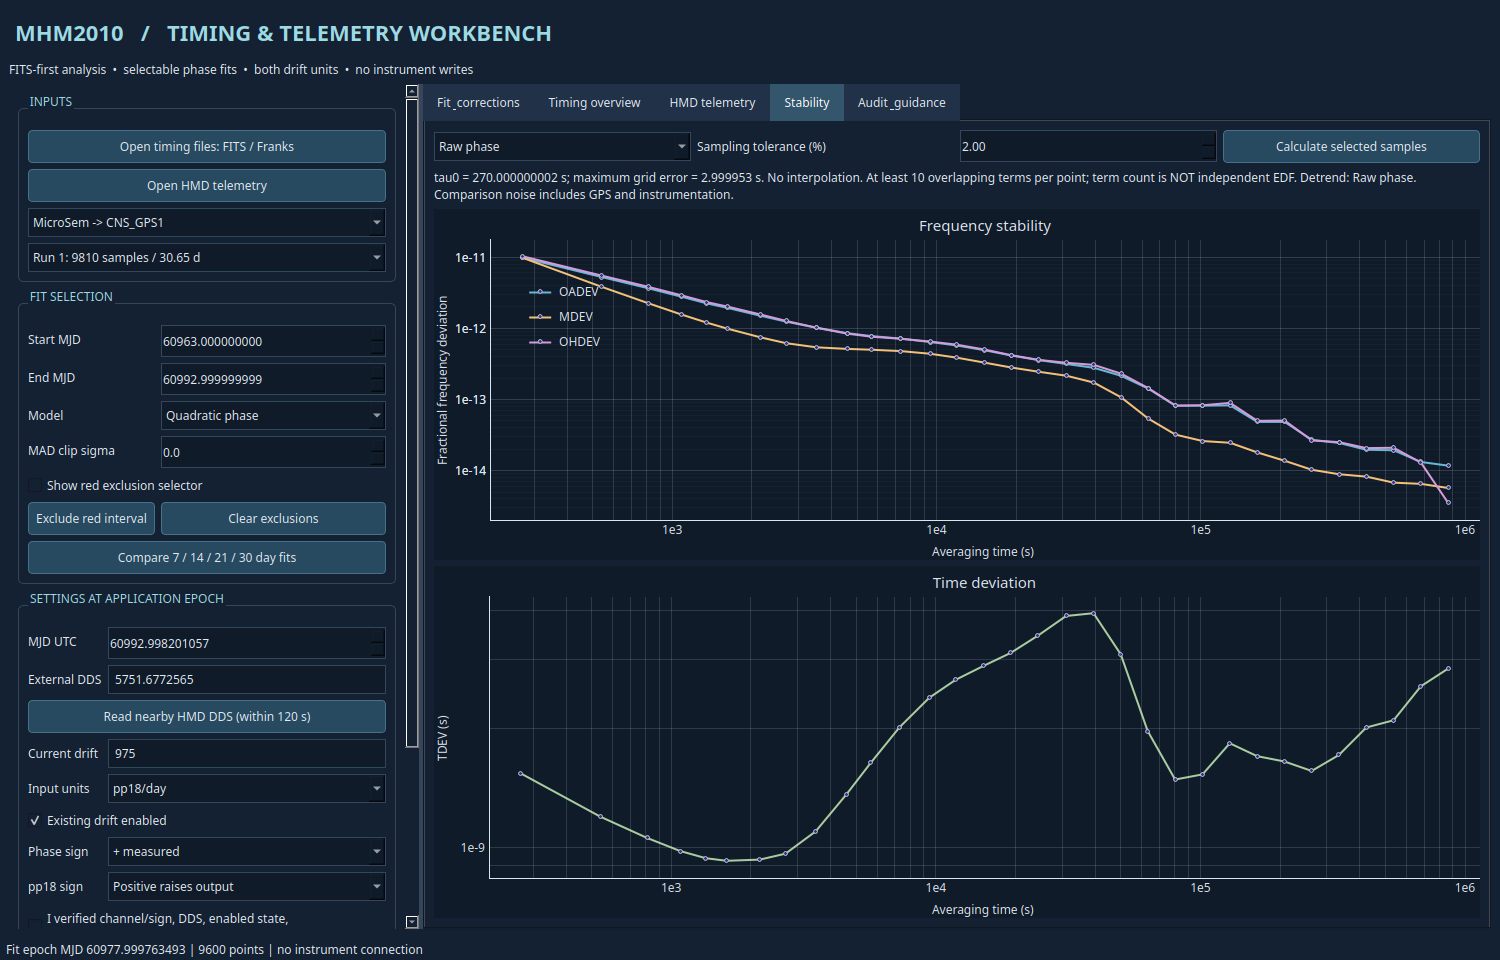
\includegraphics[width=.94\linewidth]{../validation/gui_stability.png}
\end{center}

\subsection{Stable32 files}
\texttt{raw.PHD} holds phase seconds and \texttt{raw.FRD} holds fractional
frequency derived from successive phase samples. The frequency record has one
fewer point. Fit-residual versions are written separately. The headers contain
type, point count and tau; companion CSV/JSON files retain original timestamps,
units, tolerance checks and export decisions \stablemanual.

Stable32 treats embedded zeros as gaps. Actual zeros are exported as
\texttt{1e-99}, following the manual's recommendation; replacements are counted
in the sidecar \stablemanual. Do not use its gap-fill controls to disguise a
nonuniform or incomplete input record.
\clearpage

\section{Output package and reproducibility}
\begin{longtable}{@{}p{.35\linewidth}p{.60\linewidth}@{}}
\toprule
Output & Meaning\\
\midrule
\texttt{analysis.vszh5} & Native HDF5 document, typed datasets and Veusz plotting script.\\
\texttt{analysis.json} & Fit, coefficients, conditional covariance, settings, both drift units, provenance and warnings.\\
\texttt{phase\_and\_fit.csv} & All input timing samples, model, residual, selection and fit masks.\\
\texttt{telemetry\_overlap.csv} & HMD rows overlapping the selected timing interval, if present.\\
\texttt{stability.csv} & Estimator, tau, deviation and overlapping-term count.\\
\texttt{raw.PHD / raw.FRD} & Optional uniform-record Stable32 phase and fractional frequency.\\
\texttt{fit\_residual.*} & Separately identified residual stability inputs.\\
\texttt{review.md} & Human-readable advisory summary and reference table.\\
\bottomrule
\end{longtable}

The HDF5 document is written using the supplied writer without importing
Veusz. All measured raw pair datasets and descriptive labels are included when
the full collection is exported. Overview medians are separate datasets.
The example's externally rendered PDF is a preview, not a dependency of the
application.

Exports first build in a temporary adjacent folder and rename only after
success. An existing destination is rejected. This protects earlier results
on ordinary local filesystems; no distributed-filesystem transactional
guarantee is claimed.

\subsection{Batch operation}
\begin{lstlisting}
python analyze_maser.py --fits-directory <FITS_DIRECTORY>
  --hmd <HMD_FILE> --start 2025-10-15 --end 2025-11-14
  --derive-dds --drift 975 --sampling-tolerance .02
  --stable32 --output <NEW_OUTPUT_DIRECTORY>
\end{lstlisting}
Join the lines for the shell. The end time is exclusive. Without DDS and drift
inputs, the batch path exports measurement results without a correction
candidate. \texttt{--derive-dds} only copies an HMD setting within 120 s of the
historical application epoch; it does not retrieve present-day state.

\subsection{Writer revision}
The attached writer was version 0.0.21. A targeted test demonstrated that
\texttt{dataset\_date()} accepted multidimensional input, creating invalid
date shape or silently flattening it in resizable mode. Version 0.0.22 adds
one-dimensional validation before creating the dataset group. Valid callers
retain the same API. This is a scoped defect correction, not an exhaustive
review of every writer feature.
\clearpage

\section{Historical validation results}
The uploaded archive contains 109 FITS.GZ files and 40 measured channel pairs,
9,810 records per pair. The example selects October 15 through November 13,
2025, producing 9,600 direct MicroSem-to-CNS\_GPS1 samples. The HMD record covers
April 9, 2025, through March 25, 2026. The previously supplied July 2026 timing
files do not overlap that HMD record.

At the last selected sample, November 13, 2025, 23:57:24.571 UTC, the quadratic
fit gives frequency error \(+5.83844\times10^{-15}\), residual drift
\(-660.833\) parts in \(10^{18}\)/day and phase-residual RMS 5.405 ns.
These are computed results from the supplied files, not external instrument
specifications.

\warning{The example assumes enabled drift \(+975\) pp18/day and a positive
pp18 sign that raises output frequency. The older screenshot supplies that
example number, but does not establish its value in November. The following
candidates are historical and unapproved.}

\begin{tabular}{@{}p{.49\linewidth}r@{}}
\toprule
Quantity & Historical example\\
\midrule
HMD DDS near the last timing sample & 5751.6772565\\
Calculated DDS increment, last digits & +82.929597\\
New rounded DDS & 5751.6772648\\
New drift, pp18/day & +1635.833066\\
Equivalent new drift, DDS units/day & -23.235467\\
Nearest integer pp18/day alternative & +1636\\
Nearest integer DDS units/day alternative & -23\\
\bottomrule
\end{tabular}

\subsection{The dominant warning: fit-window sensitivity}
\begin{tabular}{@{}rrrr@{}}
\toprule
Window, d & Frequency error at common end & Drift, pp18/day & RMS, ns\\
\midrule
30 & \(+5.83844\times10^{-15}\) & -660.833 & 5.405\\
21 & \(+3.80025\times10^{-15}\) & -883.575 & 5.810\\
14 & \(+1.39421\times10^{-14}\) & +407.199 & 5.922\\
7  & \(-4.32655\times10^{-15}\) & -5454.180 & 6.970\\
\bottomrule
\end{tabular}

The drift changes sign with the fitting interval. Conditional OLS errors are
much smaller than this variation and must not be interpreted as a complete
uncertainty budget. A longer/reference-checked operating-state review is
needed before any live adjustment.

For the 30-day window, CNS2018 and CNS\_GPS2 comparisons give \(-688.966\)
and \(-652.571\) pp18/day. Similar values are useful but do not demonstrate
independent references or isolate maser aging.
\clearpage

\section{Cross-checks, testing and limitations}
\subsection{Franks/Veusz comparison}
The supplied Veusz example was read as HDF5 data, without executing its
embedded plotting script. Across 735 matching UTC-hour bins in the full
archive span, the new derived MSM--GPS comparison differs by 1.284 ns RMS
from the historical reduced values. MicroSem and CNS\_GPS1 differ by
0.852 ns and 1.004 ns RMS. Median differences are approximately zero.
The maximum absolute differences are 4, 2 and 4 ns respectively.

These small differences are consistent with nonidentical reduction windows
and rounding, but that explanation is not a proof of identical processing.
The direct raw pair remains the primary correction input. Invalid negative
MJD legacy records and all-missing channels in the exemplar were not copied.

\subsection{Automated and rendering checks}
The delivered suite has 36 passing tests on Python 3.12. Tests cover analytic
phase coefficients, DDS direction, quantization, both drift representations,
disabled drift, reversal, duplicates, gap/grid rejection, clipping, FITS
metadata/padding, Franks sentinels, GUI controls/settings, writer behavior and
export protection.

OADEV, MDEV, TDEV and OHDEV were compared with AllanTools for seeded synthetic
phase data, including contributing-term counts. The 29-page historical
\texttt{.vszh5} was opened and rendered with a separate Veusz installation.
Its PDF has page bookmarks. GUI captures document the offscreen Qt tests.

\subsection{Not validated}
\begin{itemize}
\item \textbf{Windows/bracca}: actual desktop operation and local staging were not performed.
\item \textbf{Stable32 executable}: output structure was checked, but proprietary-application import remains a site test.
\item \textbf{Installed masermon}: sign, range, precision, update cadence, persistence and firmware/version behavior remain site checks.
\item \textbf{Physical system}: no live adjustment, calibration or post-adjustment monitoring was conducted.
\item \textbf{Uncertainty}: no colored-noise confidence intervals, reference-error removal or independent maser-aging measurement is claimed.
\end{itemize}

\subsection{Repository provenance}
The RF\_Equipment\_Comms stability-tool code
\href{https://github.com/Braveheart53/RF_Equipment_Comms/tree/main/sa_stability_tool}{[5]}
and FitsAutoPlot sources \href{https://github.com/Braveheart53/FitsAutoPlot}{[6]}
were read for header, GUI and analysis conventions. The science modules in this package
are new implementations using the cited definitions, not a wholesale copy of
the signal-analyzer tool. Repository checkouts were read-only with respect
to their remotes; no push was performed.

Reviewed commits:
\begin{itemize}
\item RF\_Equipment\_Comms: \texttt{9305e94e9ad85dbdb94a3765cf0989449dc3f345}.
\item FitsAutoPlot: \texttt{36add38d973bc07e920ff70680a139241c421f7c}.
\end{itemize}
The product-page pointer is
\href{https://www.microchip.com/en-us/product/mhm-2010}{Microchip MHM-2010 [7]}.
\clearpage

\section{Appendix A: Implemented equations}
\subsection{Time, phase and polynomial fit}
Let \(t\) be elapsed SI seconds, obtained by converting UTC timestamps through
TAI, and \(d\) elapsed days from fit epoch \(t_0\). The MJD plotting conversion
is only a civil-date coordinate; it is not used for elapsed-time derivatives.
\begin{align}
t_i-t_0&=\operatorname{TAI}(\operatorname{UTC}_i)-
          \operatorname{TAI}(\operatorname{UTC}_0),&
d_i&=(t_i-t_0)/86400, \tag{A1}\\
v_i&=86400(\mathrm{MJD}_i-54832),&
h_i&=\lfloor24\,\mathrm{MJD}_i\rfloor. \tag{A2}
\end{align}
Here \(v_i\) is the Veusz seconds coordinate relative to 2009-01-01 and \(h_i\)
indexes a UTC-hour reduction bucket. Within each nonempty bucket, time and
phase are reduced by their medians:
\begin{equation}
(\widetilde{\mathrm{MJD}}_h,\widetilde{x}_h)
=\left(\operatorname{median}_{i:h_i=h}\mathrm{MJD}_i,\,
       \operatorname{median}_{i:h_i=h}x_i\right). \tag{A3}
\end{equation}

With phase coefficients in nanoseconds and \(d\) in days:
\begin{align}
\widehat{x}(d)&=10^{-9}(c_0+c_1d+c_2d^2)\ \mathrm{s}, \tag{A4}\\
y(d)&=\frac{10^{-9}}{86400}(c_1+2c_2d),&
r\equiv\frac{dy}{dd}&=\frac{2c_2\,10^{-9}}{86400}\ \mathrm{day}^{-1}. \tag{A5}
\end{align}
For a linear fit, \(c_2\) is not estimated; the drift result is withheld, not
presented as evidence of zero physical drift.

Let \(s=\max_i|d_i|\), \(A_{ij}=(d_i/s)^j\), \(b_i=10^9x_i\), and let
\(T=\operatorname{diag}(1,s^{-1},s^{-2})\), truncated for a linear fit:
\begin{align}
\widehat{\boldsymbol\beta}&=\arg\min_{\boldsymbol\beta}
 \|A\boldsymbol\beta-\mathbf b\|_2^2,&
\mathbf c&=T\widehat{\boldsymbol\beta}, \tag{A6}\\
\widehat{\sigma}^2&=\frac{\sum_i e_i^2}{N-p},&
C_c&=T\left[\widehat{\sigma}^2(A^\mathsf{T}A)^{-1}\right]T^\mathsf{T},
 & e_i&=b_i-(A\widehat{\boldsymbol\beta})_i. \tag{A7}
\end{align}
Here \(p\) is coefficient count. The reported fit scatter and conditional
uncertainties are:
\begin{align}
\mathrm{RMS}_{\mathrm{ns}}&=\sqrt{\frac1N\sum_i e_i^2},&
\sigma_y&=\frac{10^{-9}}{86400}\sqrt{\mathbf g^\mathsf{T}C_c\mathbf g},
 &\mathbf g&=(0,1,2d)^\mathsf{T}, \tag{A8}\\
\sigma_r&=\frac{2\,10^{-9}}{86400}\sqrt{(C_c)_{22}}. \tag{A9}
\end{align}
They assume IID residuals conditional on the chosen fit; they do not represent
a full timing-standard uncertainty.
\clearpage

\subsection{Clipping, continuity and channel convention}
Optional clipping uses median-centered residuals and a robust scale:
\begin{equation}
M=\operatorname{median}(e),\quad
S=1.4826\,\operatorname{median}|e-M|,\quad
\text{retain }i\ \text{if}\ |e_i-M|\le kS. \tag{A10}
\end{equation}
There are at most eight clipping passes, followed by a final refit. \(k=0\)
disables clipping. A fitting run is split at gaps exceeding five median
timestamp intervals:
\begin{equation}
\Delta\mathrm{MJD}_i>5\operatorname{median}(\Delta\mathrm{MJD}). \tag{A11}
\end{equation}
These are software heuristics, not manufacturer operating limits.

For ideal pulse arrival times and clock time errors relative to the same
reference:
\begin{equation}
\Delta t_{A\rightarrow B}=t_{\mathrm{arrival},B}-t_{\mathrm{arrival},A}
=x_A-x_B,\qquad x_{\mathrm{maser-ref}}=\epsilon\,\Delta t,\quad
\epsilon\in\{-1,+1\}. \tag{A12}
\end{equation}
Fixed cable offsets affect the constant phase term; changing delays can affect
slope and drift and are not removed automatically.

\subsection{DDS correction and both drift units}
The manufacturer relationship is \manual:
\begin{equation}
f_o=\frac{f_m}{D},\qquad D=284.08+aN,\qquad a=2\times10^{-7}. \tag{A13}
\end{equation}
For old DDS \(N\), measured residual fractional frequency \(y\), and
least-significant DDS step \(q=10^{-7}\):
\begin{align}
k_N&=\frac{a}{D},&
\frac{\delta f_o}{f_o}&\simeq-k_N\delta N,&
g_{\mathrm{digit}}&=-k_Nq, \tag{A14}\\
\Delta N&=\frac{D}{a}y,&
N_{\mathrm{new}}&=\operatorname{round}_{q}(N+\Delta N),&
\Delta n&=\Delta N/q. \tag{A15}
\end{align}
Before rounding, the static relation exactly cancels the measured residual:
\begin{equation}
1+y_{\mathrm{new}}=(1+y)\frac{D}{D_{\mathrm{new}}},\qquad
D_{\mathrm{new}}=284.08+aN_{\mathrm{new}}. \tag{A16}
\end{equation}
The quantization residual is computed from (A16) with Decimal arithmetic.
The physical DDS rate \(v\), in last digits/day, transforms as:
\begin{equation}
v_{\mathrm{new}}=(1+y)v_{\mathrm{old}}+\frac{r}{k_Nq}. \tag{A17}
\end{equation}
Let \(P\) be the displayed pp18/day value and \(\eta=+1\) when positive \(P\)
raises output frequency, or \(-1\) when it raises DDS:
\begin{align}
v_{\mathrm{old}}&=-\frac{\eta P_{\mathrm{old}}10^{-18}}{k_Nq},&
P_{\mathrm{new}}&=-\eta\,v_{\mathrm{new}}\,k_{N,\mathrm{new}}q\,10^{18}, \tag{A18}\\
P_{\mathrm{new}}&\simeq P_{\mathrm{old}}-
       \frac{\eta r\,10^{18}}{1+y},&
k_{N,\mathrm{new}}&=a/D_{\mathrm{new}}. \tag{A19}
\end{align}
The code reports the rounded-DDS conversion in the both-units table.
An inactive old drift uses \(v_{\mathrm{old}}=0\). These equations describe
the local rate at the application epoch, not undocumented firmware scheduling.
\clearpage

\subsection{Rounding, uniformity and Stable32 conversion}
For nearest-integer drift alternatives:
\begin{align}
\delta r_v&=-(\operatorname{round}v_{\mathrm{new}}-v_{\mathrm{new}})
               k_{N,\mathrm{new}}q, \tag{A20}\\
\delta r_P&=\eta(\operatorname{round}P_{\mathrm{new}}-P_{\mathrm{new}})10^{-18}.
 \tag{A21}
\end{align}

For a record of \(N\) samples, interval tolerance \(\rho\), and time coordinates
from (A1), the validation is:
\begin{align}
\tau_0&=\frac{t_{N-1}-t_0}{N-1},&
\max_i\left|\frac{t_{i+1}-t_i}{\tau_0}-1\right|&\le\rho, \tag{A22}\\
\max_i|t_i-t_0-i\tau_0|&\le\rho\tau_0,&
0&<\rho\le0.05. \tag{A23}
\end{align}
At least eight finite matching samples are required. No missing interval is
compressed or interpolated. Stable32 fractional frequency and actual-zero
encoding are:
\begin{equation}
\overline y_i=\frac{x_{i+1}-x_i}{\tau_0},\qquad
z_{\mathrm{export}}=
\begin{cases}10^{-99},&z=0\ \text{(actual observation)},\\z,&z\ne0.\end{cases}
\tag{A24}
\end{equation}
The zero convention follows Stable32's documented gap handling \stablemanual.

\subsection{Stability estimators}
Let \(\tau=m\tau_0\), with integer \(m\ge1\), and \(x_i\) phase seconds.
All sums are over valid overlapping terms of a validated complete record.
The implementations follow NIST SP 1065 \nist:
\begin{align}
\sigma_y^2(\tau)&=
\frac{\sum_{i=0}^{N-2m-1}(x_{i+2m}-2x_{i+m}+x_i)^2}
     {2\tau^2(N-2m)}, \tag{A25}\\
\operatorname{mod}\sigma_y^2(\tau)&=
\frac{\displaystyle\sum_{j=0}^{N-3m}
 \left[\sum_{i=j}^{j+m-1}(x_{i+2m}-2x_{i+m}+x_i)\right]^2}
 {2m^2\tau^2(N-3m+1)}, \tag{A26}\\
\sigma_x(\tau)&=\frac{\tau}{\sqrt3}\operatorname{mod}\sigma_y(\tau), \tag{A27}\\
\sigma_H^2(\tau)&=
\frac{\displaystyle\sum_{i=0}^{N-3m-1}
(x_{i+3m}-3x_{i+2m}+3x_{i+m}-x_i)^2}
{6\tau^2(N-3m)}. \tag{A28}
\end{align}
The displayed OADEV, MDEV and OHDEV are square roots of the respective
variances. TDEV is (A27). Averaging factors are log-spaced integers, with
duplicates removed and at least ten contributing terms per reported point.
Optional detrending subtracts an OLS polynomial of order 0, 1 or 2 before
applying these equations; raw mode removes only a constant for numerical
convenience.
\clearpage

\section{Release checklist}
\begin{itemize}
\item \textbf{Code}: Python 3.12 syntax, headers, revision history and Spyder cells.
\item \textbf{GUI}: qtpy/PySide6, pyqtgraph, fitting, overview, HMD, stability and audit.
\item \textbf{Science}: explicit phase sign, epoch, both drift units, no housekeeping-only calibration.
\item \textbf{Outputs}: native HDF5, raw and reduced datasets, Stable32 and provenance.
\item \textbf{Documentation}: editable LuaLaTeX, references, equations and PDF bookmarks.
\item \textbf{Limits}: no live writes; Windows, masermon and Stable32 site tests remain.
\end{itemize}

Safran T4 i3000 implementation is not part of this release. Its planning begins
only after the MHM2010 package has been posted for download.

\section{IEEE reference table}
Online references were accessed November 3, 2026. The source URLs are retained
in full; absent DOIs or unverified publication details are not invented.

\small
\begin{longtable}{@{}p{.05\linewidth}p{.53\linewidth}p{.34\linewidth}@{}}
\toprule
Ref. & Full bibliographic entry & DOI or URL\\
\midrule
\endhead
[1] & Microsemi, \textit{Atomic Hydrogen Maser Frequency Standard Model
MHM-2010 User's Guide}, doc. 75666-201, rev. J, Oct. 2014, pp. 14, 20, 44.
& \url{https://www.gb.nrao.edu/~fghigo/timer/MSMmaser/Maser_UG_75666-201_Rev_J.PDF}\\[5pt]
[2] & W. J. Riley, \textit{Handbook of Frequency Stability Analysis},
NIST Special Publication 1065, Jul. 2008.
& \url{https://tf.nist.gov/general/pdf/2220.pdf}\\[5pt]
[3] & W. J. Riley, \textit{Stable32 User Manual}, ver. 1.54,
Sep. 7, 2008.
& \url{http://www.stable32.com/Manual154.pdf}\\[5pt]
[4] & F. Ghigo, ``Clock Monitoring at Green Bank,'' National Radio Astronomy
Observatory, web page; revision information varies within the page.
& \url{https://www.gb.nrao.edu/~fghigo/timer/time_logging.html}\\[5pt]
[5] & W. W. Wallace, ``RF\_Equipment\_Comms: sa\_stability\_tool,''
GitHub repository, reviewed commit
\texttt{9305e94e9ad85dbdb94a3765cf0989449dc3f345}, accessed Nov. 3, 2026.
& \url{https://github.com/Braveheart53/RF_Equipment_Comms/tree/main/sa_stability_tool}\\[5pt]
[6] & W. W. Wallace, ``FitsAutoPlot,'' GitHub repository, reviewed commit
\texttt{36add38d973bc07e920ff70680a139241c421f7c}, accessed Nov. 3, 2026.
& \url{https://github.com/Braveheart53/FitsAutoPlot}\\[5pt]
[7] & Microchip Technology, ``MHM-2010,'' product web page, publication date
not stated, accessed Nov. 3, 2026.
& \url{https://www.microchip.com/en-us/product/mhm-2010}\\
\bottomrule
\end{longtable}
\normalsize

\end{document}
